\chapter{The Physical Properties of Fluids}\label{c1}
\section{Notation}
The notations in these notes differ from the book in a few cases.
\begin{itemize}
\item The symbol $\sigma_{ij}$ denotes both the tensor itself as well as its $ij$th component. Sometimes, we will denote the tensor itself as $\{\sigma_{ij}\}$.

\item We use standard notation of thermodynamics instead of the one in the book. Thus, internal energy is $U$, enthalpy is $H$ and Helmholtz free energy is $A$. Further, we will follow 
the convention of using capital letters for extensive quantities and small letters for intensive ones. Further, the inexact differential of a function, say $Q$, is denoted by $\dbar Q$ 
while $dS$ denotes exact differential of $S$.

\item We denote average of a quantity $x$ as $\langle x \rangle$ instead of $\bar{x}$.

\item Components of velocity vector are $u_1, u_2, u_3$ instead of $u, v, w$.

\item The azimuthal angle in cylindrical and spherical polar coordinates is denoted by $\varphi$.

\end{itemize}

\section{Volume forces and surface forces action on a fluid}\label{c1s3}
\begin{itemize}
\item The stress tensor $\sigma_{ij}$ is symmetric unless the fluid has a natural body couple. We can prove it by considering the couple (torque) $\vec{N}$ on a small volume element
of the fluid, due only to surface forces. If $\vec{F}$ is the force density then
\[
\vec{N} = \int \vec{r} \vp \vec{F} dV
\]
If the volume element is small enough so that $\vec{F}$ is almost uniform over it, the couple is of $O(r^4) = O(V^{4/3})$. In terms of the stress tensor, 
\begin{equation}\label{c1s3e1}
N_i = \int \epsilon_{ijk}r_j \sigma_{kl} n_l dA
\end{equation}
Using divergence theorem,
\begin{eqnarray}
N_i &=& \int \pdts{\epsilon_{ijk}r_j \sigma_{kl}}{r_l} dV \nonumber \\
 &=& \int \epsilon_{ijk}\left(\delta_{jl}\sigma_{kl} + r_k \pdt{\sigma_{kl}}{r_l}\right)dV \nonumber \\
 &=& \int \epsilon_{ijk}\sigma_{jk} dV + \int \epsilon_{ijk}r_k\pdt{\sigma_{kl}}{r_l} dV \label{c1s3e2}
\end{eqnarray}
From \eqref{c1s3e1} it is clear that if the volume element is small enough for $\sigma_{ij}$ and $\partial\sigma_{kl}/\partial r_l$ to vary slowly over it then $N_i$ is $O(V^{4/3})$. By 
the same reasoning, the first term on the right hand side of \eqref{c1s3e2} is $O(V)$ while the second term is $O(V^{4/3})$. Thus, in the limit of $V$ going to zero, left hand side of 
\eqref{c1s3e2} and the second term on its right hand side vanish faster than the first term on its right hand side. Therefore, the equation can continue to be valid in this limit only if 
the first term on its right hand side is zero, which can happen for an arbitrary volume element only if
\begin{equation}\label{c1s3e3}
\epsilon_{ijk}\sigma_{jk} = 0
\end{equation}
\begin{itemize}
\item If there is a natural body couple, as in the case of a polarized fluid, then $\sigma_{ij}$ will not vary slowly over the volume element. In fact, it will end up being of the order 
$O(V^x)$ for some real number $x$. In that case, the right hand side of \eqref{c1s3e1} is $O(V^{1 + x})$, first term on right hand side of \eqref{c1s3e2} is $O(V^{1 + x})$ and the
second term is $O(V^{1 + x})$. Since all terms are of the same order, we cannot draw any conclusion on the nature of $\sigma_{ij}$.
\item We will now show that \eqref{c1s3e3} implies $\sigma_{ij} = \sigma_{ji}$. Since $\epsilon_{ijk} = 0$ if any two or more indices are equal, the left hand side of \eqref{c1s3e3} is
\[
(\sigma_{23} - \sigma_{32})\uvec{1} + (\sigma_{31} - \sigma_{13})\uvec{2} + (\sigma_{12} - \sigma_{21})\uvec{3} = 0
\]
The symmetry of the tensor follows immediately.
\item From the preceding equation it is clear that if the stress tensor is symmetric then the total couple on a volume element of a fluid is zero. We will use this fact in section 
\ref{c1s4}.
\end{itemize}
\end{itemize}

\section{Mechanical equilibrium of a fluid}\label{c1s4}
\begin{itemize}
\item A volume element of a fluid is in equilibrium if the total force and couple on it vanish. We saw in section \ref{c1s3} that the symmetry of stress tensor leads to vanishing of 
torque. Now, the total force on the volume element is
\[
\int\rho F_i dv + \int\sigma_{ij}n_j dA
\]
For a static fluid, $\sigma_{ij} = -p\delta_{ij}$. Using divergence theorem on the 
second term,
\begin{eqnarray*}
\int \sigma_{ij}n_j dA &=& \int \frac{\partial\sigma_{ij}}{\partial x_j} dV \\
 &=& -\int \pdt{p\delta_{ij}}{x_j} dV \\
 &=& -\int \pdt{p}{x_j}\delta_{ij} dV + 0 \\
 &=& -\int \grad{p}dV
\end{eqnarray*}
Thus, the total force on the volume element is
\[
\int \left(\rho\vec{F} - \grad{p}\right) dV
\]
It is zero for an arbitrary volume element if
\begin{equation}\label{c1s4e1}
\rho\vec{F} = \grad{p}
\end{equation}
\begin{itemize}
\item Since $\grad{p}$ is in the direction of $\vec{F}$, $p$ is constant along a direction perpendicular to it. Thus, the level surfaces of $p$ are all normal to $\vec{F}$.
\item Equation \eqref{c1s4e1} tells that a fluid is in mechanical equilibrium only for those arrangements of $\rho$ and $\vec{F}$ for which their product is a gradient of a scalar field, 
called the pressure.
\item If $\vec{F}$ is a conservative force, then \eqref{c1s4e1} can be written as 
\begin{equation}\label{c1s4e2}
-\rho\grad{\Psi} = \grad{p},
\end{equation}
where $\Psi$ is the potential of $\vec{F}$. Taking curl of both sides,
\begin{equation}\label{c1s4e3}
\grad{\rho} \vp \grad{\Psi} = 0
\end{equation}
or that $\grad{\rho}$ is parallel to $\grad{\Psi}$. From \eqref{c1s4e2} $\grad{\Psi}$ is also parallel to $\grad{p}$. Thus, a fluid is in mechanical equilibrium when the level surfaces of
the three scalar fields, $\rho$, $p$ and $\Psi$ are identical.
\item We will now show that \eqref{c1s4e2} is equivalent to $\rho = -dp/d\Psi$. We start with
\[
dp = \pdt{p}{x}dx + \pdt{p}{y}dy + \pdt{p}{z}dz
\]
or,
\[
\td{p}{\Psi} = \pdt{p}{x}\pdt{x}{\Psi} + \pdt{p}{y}\pdt{y}{\Psi} + \pdt{p}{z}\pdt{z}{\Psi}
\]
or,
\[
\td{p}{\Psi} = \pdt{p}{x}\frac{1}{\pdt{\Psi}{x}} + \pdt{p}{y}\frac{1}{\pdt{\Psi}{y}} + \pdt{p}{z}\frac{1}{\pdt{\Psi}{z}}
\]
Define
\[
\vec{\Phi} = \frac{\uvec{x}}{\pdt{\Psi}{x}} + \frac{\uvec{y}}{\pdt{\Psi}{y}} + \frac{\uvec{z}}{\pdt{\Psi}{z}}
\]
Therefore,
\[
\td{p}{\Psi} = \grad{p}\cdot\vec{\Phi}
\]
Further, $\vec{\Phi}\cdot\grad{\Psi} = 1$. Therefore, if we take a dot product of equation \eqref{c1s4e2} with $\vec{\Psi}$, we get
\begin{equation}\label{c1s4e4}
\td{p}{\Psi} = -\rho
\end{equation}
\item In the event, $\rho$ is independent of $p$, as in the case of liquids under moderate pressures, we can integrate \eqref{c1s4e4} to get $p = p_0 - \rho\Psi$. If $\Psi$ refers to
gravitational field in a laboratory, $p = p_0 - \rho gz$.
\end{itemize}

\item Consider a solid body of density $\rho_s$ immersed in a fluid of density $\rho_f$. It experiences force due to earth's gravity ($\vec{f}_1$) and due to pressure of the surrounding 
fluid ($\vec{f}_2$). The latter force is given by 
\[
\vec{f}_2 = -\int p(\vec{x})\un dA = -\int \grad{p} dV,
\]
the integral being over the surface of the body. If we imagine that the portion of body immersed in the fluid is replaced by an equivalent volume of fluid, keeping the fluid in mechanical 
equilibrium, then by equation \eqref{c1s4e1}, 
\[
\vec{f}_2 = -\int_{V_i} \rho_f\vec{F}dV,
\]
where $V_i$ is the volume of the immersed part of the solid. The force $\vec{f}_1$ on the solid is
\[
\vec{f}_1 = \int_{V_t} \rho_s\vec{F}dV,
\]
where $V_t$ is the total volume of the solid and hence the total force is
\begin{equation}\label{c1s4e5}
\vec{f} = \int_{V_t} \rho_s\vec{F}dV - \int_{V_i} \rho_f\vec{F}dV
\end{equation}
This is Archimedes's principle that the solid body immersed in a fluid experiences a \enquote*{buoyancy} equivalent to the \enquote*{weight} of the displaced fluid.
\begin{itemize}
\item If the body is completely immersed in the fluid and if $\rho_s > \rho_f$ then there will still be a net downward force on the body. It can be balanced either by suspending the body
by a string, or if the body is magnetic, by a magnetic field.
\end{itemize}

\item Consider a fluid in a vessel rotating around the $z$ axis. The axes are chosen such that the gravitational force is along the negative $z$ axis. In the frame of reference of the
rotating fluid, the potential field, $\Psi$, is that of gravity and centrifugal forces. Thus,
\[
\Psi = gz - \frac{\Omega^2}{2}(x^2 + y^2)
\]
The level surface of $\Psi$ is given by $\Psi = c$, for some constant $c$. The equation of level surface is
\[
gz - \frac{\Omega^2}{2}(x^2 + y^2) = c
\]
or
\[
z = \frac{\Omega^2}{2g}(x^2 + y^2) + \frac{c}{g}
\]
This is the equation of an \href{https://en.wikipedia.org/wiki/Paraboloid}{elliptic paraboloid}, symmetric around the $z$ axis and whose bottom point is at $(0, 0, c/g)$.

\item If a solid body of density $\rho_s$ can stay at rest immersed in a fluid of density $\rho_l$ then, since the net force on it is zero, from equation \eqref{c1s4e5},
\begin{equation}\label{c1s4e6}
\int_{V_t} \rho_s gdV = \int_{V_i} \rho_f gdV
\end{equation}
If the body is at rest in a rotating fluid, then we have
\[
\int_{V_t}\left(\rho_s\vec{g} + \rho_s\Omega^2(x\uvec{x} + y\uvec{y})\right)dV - \int_{V_i}\left(\rho_f\vec{g} + \rho_f\Omega^2(x\uvec{x} + y\uvec{y})\right)dV = 0
\]
Using \eqref{c1s4e6},
\[
\int_{V_t}\rho_s \Omega^2(x\uvec{x} + y\uvec{y}) dV - \int_{V_i}\rho_f \Omega^2(x\uvec{x} + y\uvec{y}) dV = 0
\]
Now, let us assume that the body is completely immersed in the fluid in such a way that the net vertical force on it is zero, either by suspending it by a string or by magnetic field. In
that case, $V_t = V_i$ and the above equation because,
\[
\int_{V_t}(\rho_s - \rho_f)\Omega^2(x\uvec{x} + y\uvec{y}) dV = 0
\]
Since we assumed that $\rho_s > \rho_f$, this equation can be satisfied only if $x = y = 0$, or if the body is at the center of the vessel.

\item Pressure inside a self-gravitating star of uniform density. Pressure distribution if given by
\[
\frac{d}{dr}\left(\frac{r^2}{\rho}\frac{dp}{dr}\right) = -4\pi Gr^2\rho
\]
If $\rho=\rho_0$ is a constant, the equation simplifies to
\begin{equation}\label{c1s4e7}
\frac{d^2p}{dr^2} + \frac{2}{r}\frac{dp}{dr} = -4\pi G\rho_0^2
\end{equation}
The corresponding homogeneous equation is
\[
\frac{d^2p}{dr^2} + \frac{2}{r}\frac{dp}{dr} = 0
\]
It can be solved by first putting $q=dp/dr$ in which case, it becomes $dq/dr + (2/r)q=0$. Its solution is $q=K_1/r^2$, where $K_1$ is a constant of integration. In terms of 
$p(r)$, it can be solved further to get
\[
p_0(r) = -\frac{K_1}{r} + K_2
\]
where the subscript $0$ indicates solution of the homogeneous equation and $K_2$ is another constant of integration. The particular solution $p_1(r)$ can be assumed to be of the form
$c_0 + c_1r + c_2r^2$ where $c_0$, $c_1$ and $c_2$ are constants. Substituting $p_1(r)$ in equation \eqref{c1s4e7}, we get $6c_2 + 2c_1/r + 4\pi G\rho_0^2 = 0$. If this equation has to
be true for all $r$, we should have $c_1 = 0$ and $c_2 = -2/3 \pi G\rho_0^2$. Thus the complete solution of equation \eqref{c1s4e7} is
\[
p(r) = -\frac{K_1}{r} + K_2 -\frac{2}{3}\pi G\rho_0^2 r^2
\]
This solution is subject to two boundary conditions:
\begin{itemize}
\item[(a)] $p(0)$ should be finite and 
\item[(b)] $p(a) = 0$ where $a$ is the radius of the star.
\end{itemize}
The first condition implies $K_1 = 0$ and the second one implies $K_2 = -2/3 \pi G\rho_0^2 a^2$. Thus the pressure distribution is given by
\[
p(r) = \frac{2}{3}\pi G\rho_0^2 (a^2 - r^2)
\]

\item A polytropic process is a quasi-static process in which the specific heat of a substance remains constant\cite{chandrasekhar1958introduction}. \footnote{This solution largely 
follows the one mentioned in Chandrasekhar's book.} Along a polytropic change of a substance $pv^m = C$, where $p$ is its pressure, $v$ is its specific volume, $m$ and $C$ are constants. 
In terms of density $\rho = v^{-1}$, $p = C\rho^{m}$. If we introduce $n = (m - 1)^{-1}$, then we have
\[
p = C\rho^{1 + 1/n}
\]
We will solve the equation of equilibrium for a self-gravitating star
\begin{equation}\label{c1s4e8}
\frac{1}{r^2}\frac{d}{dr}\left(\frac{r^2}{\rho}\frac{dp}{dr}\right) = -4\pi G\rho
\end{equation}
for polytropic relation with $n = 5$. The solution requires a series of transformations, the first of which is 
\begin{equation}\label{c1s4e9}
\rho = \lambda\theta^n,
\end{equation}
where $\lambda$ is, at the moment, an arbitrary constant. In terms of $\theta$, the polytropic relation becomes 
\begin{equation}\label{c1s4e9a}
p = C\lambda^{(n+1)/n}\theta^{n+1}
\end{equation}
and equation \eqref{c1s4e8} becomes
\begin{equation}\label{c1s4e10}
\frac{C\lambda^{1/n - 1}(n + 1)}{4\pi G}\frac{1}{r^2}\frac{d}{dr}\left(r^2\td{\theta}{r}\right) = -\theta^n
\end{equation}
Introduce a new dimensionless variable $\xi = r/b$ to transform the above equation to,
\[
\frac{C\lambda^{1/n - 1}(n + 1)}{4\pi G}\frac{1}{b^2}\frac{1}{\xi^2}\frac{d}{d\xi}\left(\xi^2\td{\theta}{\xi}\right) = -\theta^n
\]
If we choose
\begin{equation}\label{c1s4e11}
b^2 = \frac{C\lambda^{1/n - 1}(n + 1)}{4\pi G},
\end{equation}
we get
\begin{equation}\label{c1s4e12}
\frac{1}{\xi^2}\frac{d}{d\xi}\left(\xi^2\td{\theta}{\xi}\right) = -\theta^n
\end{equation}
This is the Lane-Emden equation for index $n$. Its solutions, subject to the boundary conditions $\theta(0) = 1$ and $\theta^\op(0) = 0$, prime denoting differentiation with respect to 
$\xi$, are called Lane-Emden functions of index $n$. A further transformation $x = 1/\xi$, changes \eqref{c1s4e12} to
\begin{equation}\label{c1s4e13}
x^4\frac{d^2\theta}{dx^2} = -\theta^n
\end{equation}
Equation \eqref{c1s4e13} has a solution of the form $\theta(x) = a_1x^k$, where $a_1$ is a constant if
\begin{eqnarray}
k + 2&=& nk \label{c1s4e13a} \\
k(1 - k) &=& a_1^{n-1} \label{c1s4e13b}
\end{eqnarray}
which on simplification give
\begin{eqnarray}
k &=& \frac{2}{n - 1} \label{c1s4e14} \\
a_1 &=& \left[\frac{2(n - 3)}{(n - 1)^2}\right]^{1/(n - 1)} \label{c1s4e15}
\end{eqnarray}
Thus,
\begin{equation}\label{c1s4e16}
\theta(x) = \left[\frac{2(n - 3)}{(n - 1)^2}\right]^{1/(n - 1)} x^{\frac{2}{n - 1}}
\end{equation}
is a singular solution of \eqref{c1s4e12}. To get a general solution, we seek a function $z(x)$ such that $\theta(x) = Ax^k z(x)$ is a solution of \eqref{c1s4e12}. $A$ is an arbitrary 
constant. Substituting this form
in \eqref{c1s4e13} we get,
\begin{equation}\label{c1s4e17}
x^2\frac{d^2z}{dx^2} + 2kx\td{z}{x} + k(k - 1)z + A^{n - 1}z^n = 0
\end{equation}
A further transformation $x = e^t$ takes it to
\begin{equation}\label{c1s4e18}
\frac{d^2z}{dt^2} + (2k - 1)\td{z}{t} + k(k - 1)z + A^{n - 1}z^n = 0
\end{equation}
Since $A$ was arbitrary, we choose it to be $a_1$. Therefore, using \eqref{c1s4e13b} we get
\begin{equation}\label{c1s4e19}
A^{n - 1} = k(1 - k)
\end{equation}
Equation \eqref{c1s4e18}, therefore, becomes
\begin{equation}\label{c1s4e20}
\frac{d^2z}{dt^2} + (2k - 1)\td{z}{t} - k(k - 1)z(1 - z^{n - 1}) = 0
\end{equation}
Using \eqref{c1s4e14}, we get
\begin{equation}\label{c1s4e21}
\frac{d^2z}{dt^2} + \frac{5 - n}{n - 1}\td{z}{t} - \frac{2(n - 3)}{(n - 1)^2}z(1 - z^{n - 1}) = 0
\end{equation}
We now specialize to $n = 5$ so that
\begin{equation}\label{c1s4e22}
\frac{d^2z}{dt^2} - \frac{z}{4}(1 - z^4) = 0
\end{equation}
or
\[
\td{z}{t}\frac{d^2z}{dt^2} = \frac{z}{4}(1 - z^4)\td{z}{t}
\]
or
\[
\left(\td{z}{t}\right)^2 = \frac{z^2}{4} - \frac{z^6}{12} + 2D,
\]
where $2D$ is a constant of integration. It is arbitrarily set to zero so that
\[
\frac{dz}{z\sqrt{1 - \frac{z^4}{3}}} = -\frac{dt}{2}
\]
We can integrate it if we put 
\begin{equation}\label{c1s4e23}
\frac{z^4}{3} = \sin^2\zeta
\end{equation}
to get
\[
\csc\zeta d\zeta = -dt
\]
or
\[
-\ln(\csc\zeta + \cot\zeta) = -t + \alpha,
\]
or
\begin{equation}\label{c1s4e24}
\tan\left(\frac{\zeta}{2}\right) = Ke^{-t},
\end{equation}
$K$ being a constant of integration. From \eqref{c1s4e23} and \eqref{c1s4e24},
\begin{equation}\label{c1s4e25}
z = \left[\frac{12K^2e^{-2t}}{(1 + K^2e^{-2t})^2}\right]^{1/4}
\end{equation}
Since we chose $A = a_1$,
\begin{equation}\label{c1s4e26}
\theta(x) = a_1x^kz(x) = a_1x^k \left[\frac{12K^2e^{-2t}}{(1 + K^2e^{-2t})^2}\right]^{1/4}
\end{equation}
Since we specialized to $n=5$, from equations \eqref{c1s4e14} and \eqref{c1s4e15}, we get
\begin{eqnarray}
k &=& \frac{1}{2} \label{c1s4e27} \\
a_1 &=& \frac{1}{4^{1/4}} \label{c1s4e28}
\end{eqnarray}
Using \eqref{c1s4e27} and \eqref{c1s4e27} in \eqref{c1s4e26}, and noting that $x = \xi^{-1} = e^t$, we get
\begin{equation}\label{c1s4e29}
\theta(\xi) = \left[\frac{3K^2}{(1 + K^2\xi^2)^2}\right]^{1/4}
\end{equation}
Since $\theta(\xi = 0) = 1$, $3K^2 = 1$ and hence,
\begin{equation}\label{c1s4e30}
\theta(\xi) = \left[\frac{1}{(1 + \xi^2/3)^2}\right]^{1/4} = \frac{1}{(1 + \xi^2/3)^{1/2}}
\end{equation}
This equation is also reported on the \href{http://mathworld.wolfram.com/Lane-EmdenDifferentialEquation.html}{Wolfram} website.
Putting $n = 5$ in \eqref{c1s4e9a} and using the above equation in it, we get
\begin{equation}\label{c1s4e31}
p(\xi) = C\lambda^{6/5}\theta^6 = \frac{C\lambda^{6/5}}{(1 + \xi^2/3)^3}
\end{equation}
Since $\xi = r/b$,
\begin{equation}\label{c1s4e32}
p(r) = \frac{27b^6C\lambda^{6/5}}{(3b^2 + r^2)^3}
\end{equation}
Putting $n = 5$ in \eqref{c1s4e11},
\[
\lambda^{2/5} = \sqrt{\frac{3C}{2\pi G}}\frac{1}{b}
\]
Using this expression in \eqref{c1s4e32},
\begin{eqnarray*}
p(r) &=& \frac{27b^3C}{(3b^2 + r^2)^3} \frac{(3C)^{3/2}}{(2\pi G)^{3/2}} \\
 &=& \frac{27(b\sqrt{3})^3 C^{5/2}}{(2\pi G)^{3/2}} \frac{1}{((b\sqrt{3})^2 + r^2)^3}
\end{eqnarray*}
Let $a = b\sqrt{3}$ so that,
\begin{equation}\label{c1s4e33}
p(r) = \frac{27a^3 C^{5/2}}{(2\pi G)^{3/2}} \frac{1}{(a^2 + r^2)^3}
\end{equation}
\end{itemize}

\subsection{Exercises}
\begin{enumerate}
\item Choose the coordinate axes such that the vessel rotates about the $y$ axis and the gravity is along the negative $z$ axis. Therefore, force on unit volume element of the fluid is
\[
\vec{F} = -g\uvec{z} + \Omega^2(x\uvec{x} + z\uvec{z})
\]
The corresponding potential is
\[
\Psi(\vec{r}) = gz - \frac{\Omega^2}{2}(x^2 + z^2) = -\frac{\Omega^2}{2}x^2 - \frac{\Omega^2}{2}\left(z^2 - \frac{2gz}{\Omega^2}\right)
\]
or,
\[
\Psi(\vec{r}) = -\frac{\Omega^2}{2}x^2 - \frac{\Omega^2}{2}\left(z - \frac{g}{\Omega^2}\right)^2 + \frac{g^2}{2\Omega^2}
\]
Level surfaces of $\Psi(\vec{r}) = -K$ have equation
\[
\frac{\Omega^2}{2}x^2 + \frac{\Omega^2}{2}\left(z - \frac{g}{\Omega^2}\right)^2 = K + \frac{g^2}{2\Omega^2}
\]
or
\[
x^2 + \left(z - \frac{g}{\Omega^2}\right)^2 = \frac{2}{\Omega^2}\left(K + \frac{g^2}{2\Omega^2}\right)
\]
Since the level surfaces of pressure, $\Psi$ and $\rho$ coincide when the fluid is in mechanical equilibrium, above equation also describes level surfaces of $p$ for every value of $K$.
Further, the equation describes a family of cylinders whose axis is parallel to the $y$ axis and is at a height $g/\Omega^2$ above it.

\item Density distribution is given by $\rho = \rho_c(1 - \beta r^2)$. Pressure distribution if given by equation \eqref{c1s4e7},
\[
\frac{d}{dr}\left(\frac{r^2}{\rho}\frac{dp}{dr}\right) = -4\pi Gr^2\rho
\]
Substituting expression for density distribution in, we get
\begin{equation}\label{c1s4e34}
\frac{d^2p}{dr^2} + \frac{2}{r(1 - \beta r^2)}\frac{dp}{dr} + 4\pi G\rho_c^2(1 - \beta r^2) = 0
\end{equation}
The corresponding homogeneous equation is
\begin{equation}\label{c1s4e35}
\frac{d^2p}{dr^2} = -\frac{2}{r(1 - \beta r^2)}\frac{dp}{dr}
\end{equation}
If $q=dp/dr$, it can be integrated as
\begin{equation}\label{c1s4e36}
\ln|qr^2| = \ln|K_1(1-\beta r^2)|
\end{equation}
where $K_1$ is a constant of integration. Second integration gives
\begin{equation}\label{c1s4e37}
p_h(r) = -K_1\left(\frac{1}{r} + \beta r\right) + K_2
\end{equation}
where $K_2$ is the second constant of integration and the subscript h indicates the solution of the homogeneous equation. The particular integral $p_c(r)$ is found by the trial function 
\[
\sum_{k=0}^7c_kx^{7-k}
\]
Substituting this form in equation \eqref{c1s4e34} and equating coefficients of like powers of $r$ we get
\begin{eqnarray*}
c_0 &=& 0		\\
c_1 &=& -\frac{2\pi}{15}G\rho_c^2\beta^2	\\
c_2 &=& 0		\\
c_3 &=& \frac{8\pi}{15}G\rho_c^2\beta	\\
c_4 &=& 0		\\
c_5 &=& -\frac{2\pi}{3}G\rho_c^2		\\
c_6 &=& 0		\\
c_7 &=& 0	
\end{eqnarray*}
Thus the solution of \eqref{c1s4e34} is
\[
p(r) = -\frac{2\pi}{15}G\rho_c^2\beta^2r^6 + \frac{8\pi}{15}G\rho_c^2\beta r^3 - \frac{2\pi}{3}G\rho_c^2r^2 - \frac{K_1}{r} - K_1\beta r + K_2
\]
The two boundary conditions are (1) $p(0)$ should be finite and (2) $p(a)=0$. The first one requires $K_1 = 0$ while the second one gives
\[
K_2 = \frac{2\pi}{15}G\rho_c^2\beta^2a^6 - \frac{8\pi}{15}G\rho_c^2\beta a^4 + \frac{2\pi}{3}G\rho_c^2a^2
\]
The complete solution of \eqref{c1s4e34} thus is
\begin{equation}\label{c1s4e38}
p(r) = \frac{2\pi}{15}G\rho_c^2\beta^2(a^6-r^6) - \frac{8\pi}{15}G\rho_c^2\beta(a^4-r^4) +\frac{2\pi}{3}G\rho_c^2(a^2-r^2)
\end{equation}
Equation \eqref{c1s4e38} is the pressure distribution in a self-gravitating spherical star with density distribution $\rho = \rho_c(1-\beta r^2)$.
Mean density of the star is
\[
\langle\rho\rangle = \frac{3}{4\pi a^3}\int_0^a\int_0^\pi\int_0^{2\pi}\rho_c(1-\beta r^2) r^2\sin\theta dr d\theta d\phi
\]
Solving the integral we get 
\[
\langle\rho\rangle =\rho_c\left(1-\frac{3}{5}\beta a^2\right)
\]
Given that the mean density of the star is twice the surface density, that is, $\langle\rho\rangle = 2\rho_c(1 - \beta a^2)$. This condition gives $\beta=5/(7a^2)$. The total mass of such 
a star is
\[
M = \int_0^a\int_0^\pi\int_0^{2\pi}\rho_c(1-\beta r^2) r^2\sin\theta dr d\theta d\phi,
\]
after evaluating the integral and putting $\beta=5/(7a^2)$, we get
\[
M = 4\pi\rho_c\left(\frac{a^3}{3} - \frac{a^3}{7}\right) = \frac{4\pi}{3}\rho_c a^3 \frac{4}{7}
\]
A star of the same mass but with uniform mass distribution will have density $\rho_0=(4/7)\rho_c$. Pressure at the center of such a star will be
\[
p_u(r=0) = \frac{2}{3}\pi G \left(\frac{4\rho_c}{7}\right)^2 a^2 = \frac{32}{147}\pi G\rho_c^2a^2
\]
where we have used the second equation after (1.4.8) in the book with $r=0$ and the subscript \enquote*{u} indicates uniform mass distribution. Substituting $\beta=5/(7a^2)$ in 
\eqref{c1s4e38} and evaluating it at $r=0$ we get the pressure at the center of the star with mass distribution
\[
p_n(r=0) = \frac{52}{147}\pi G\rho_c^2a^2
\]
where the subscript \enquote*{n} indicates non-uniform mass distribution. Clearly 
\[
\frac{p_n(0)}{p_u(0)} = \frac{13}{8}
\]
\end{enumerate}

\section{Classical Thermodynamics}\label{c1s5}
First law of thermodynamics states that if $\dbar Q$ is the amount of heat entering a system, $\dbar W$ is the amount of work done on it then its internal energy changes as
\[
dU = \dbar Q + \dbar W
\]
Thus, although $\dbar Q$ and $\dbar W$ are in general inexact differentials, their sum is not. The first law of thermodynamics thus defines a state function, called internal energy. If
the work done (on the system) is due to compression then $\dbar W = -pdV$, so that $dU = \dbar Q - pdV$ or, equivalently
\[
\dbar Q = dU + pdV = \left(\pdt{U}{V}\right)_pdV + \left(\pdt{U}{p}\right)_Vdp + pdV
\]
Specific heat is $c = \dbar Q/dT$. Since $\dbar Q$ is an inexact differential, the value of $c$ depends on the path of transformation. At constant pressure,
\[
c_p = \left(\pdt{U}{V}\right)_p\left(\pdt{V}{T}\right)_p + p\left(\pdt{V}{T}\right)_p = \left(\pdt{U}{T}\right)_p + p\left(\pdt{V}{T}\right)_p
\]
Similarly, specific heat at constant volume is,
\[
c_V = \left(\pdt{U}{p}\right)_V\left(\pdt{p}{T}\right)_V = \left(\pdt{U}{T}\right)_V
\]
The ratio of the two specific heats, $c_p/c_V$, is usually denoted by $\gamma$. The bulk moduli of fluids under adiabatic (constant entropy, $S$) and isothermal 
(constant temperature $T$) are defined as
\begin{eqnarray*}
K_S &=& -\frac{1}{v}\left(\pdt{p}{v}\right)_S \\
K_T &=& -\frac{1}{v}\left(\pdt{p}{v}\right)_T,
\end{eqnarray*}
where $v$ is the specific volume of the material. Similarly, the two compressibilities are defined as
\begin{eqnarray*}
\kappa_S &=& -\frac{1}{v}\left(\pdt{v}{p}\right)_S \\
\kappa_T &=& -\frac{1}{v}\left(\pdt{v}{p}\right)_T
\end{eqnarray*}
The proof in the textbook considers changes in $Q$ and $T$ as vectors in phase diagram of the fluid. If $\vec{t}_i$ and $\vec{t}_a$ are unit tangents to the isothermal and adiabatic 
curves and if $\uvec{V}$ and $\uvec{p}$ are unit vectors along $V$ and $p$ axes then,
\begin{eqnarray*}
\vec{t}_i &=& m_V\uvec{V} + m_p\uvec{p} \\
\vec{t}_a &=& n_V\uvec{V} + n_p\uvec{p}
\end{eqnarray*}
Let $\vec{m}$ and $\vec{n}$ be unit normals to the isotherm and adiabatic curves.
\begin{eqnarray*}
\vec{m} &=& -m_p\uvec{V} + m_V\uvec{p} \\
\vec{n} &=& -n_p\uvec{V} + n_V\uvec{p}
\end{eqnarray*}
If $\theta_i$ and $\theta_a$ are the angles made by these tangents with the $V$ axis and if $t_i = 1$ and $t_a = 1$ are their magnitudes then
\begin{eqnarray*}
m_V &=& \cos\theta_i \\
m_p  &=& \sin\theta_i \\
n_V &=& \cos\theta_a \\
n_p  &=& \sin\theta_a
\end{eqnarray*}
Therefore,
\begin{eqnarray}
\tan\theta_i &=& \frac{m_p}{m_V} = \left(\pdt{p}{V}\right)_T \label{c1s5e0a} \\
\tan\theta_a &=& \frac{n_p}{n_V} = \left(\pdt{p}{V}\right)_S \label{c1s5e0b} 
\end{eqnarray}
Further, if 
Thus, is $\delta\vec{Q}$ and $\delta\vec{T}$ are the \enquote*{vector} changes in heat and temperature then
\begin{eqnarray*}
\delta\vec{Q} &=& n_V\delta Q\uvec{V} + n_p\delta Q\uvec{p} \\
\delta\vec{T} &=& m_V\delta T\uvec{V} + m_p\delta T\uvec{p}
\end{eqnarray*}
If $p$ is kept constant then
\[
c_p = \frac{n_V \delta Q}{m_V \delta T} 
\]
Similarly, if $V$ is kept constant then,
\[
c_V = \frac{n_p \delta Q}{m_p \delta T} 
\]
Therefore,
\[
\gamma = \frac{c_p}{c_V} = \frac{n_V}{n_p}\frac{m_p}{m_V}
\]
Using equations \eqref{c1s5e0a} and \eqref{c1s5e0b},
\[
\gamma = \left(\pdt{p}{V}\right)_S \Big/ \left(\pdt{p}{V}\right)_T
\]
The same relations hold good if we use specific volume. Thus,
\[
\gamma = \left(\pdt{p}{v}\right)_S \Big/ \left(\pdt{p}{v}\right)_T = \frac{K_S}{K_T} = \frac{\kappa_S}{\kappa_T}
\]
An easy proof of the these equations is available on \href{https://en.wikipedia.org/wiki/Relations_between_heat_capacities}{Wikipedia}\footnote{Alternatively, refer to equation 1.22 of
Huang's Statistical Mechanics\cite{huang1987statistical}}.

One of the equivalent statements of second law of thermodynamics is that the integrating factor of $\dbar Q$ is $1/T$, where $T$ is the absolute temperature. The resulting exact 
differential is of the state function called entropy $S$. Thus,
\[
dS = \frac{\dbar Q}{T}
\]
Maxwell's relations are derived from the definition of the four thermodynamic relations.
\begin{itemize}
\item Internal energy $U$ is defined as $dU = TdS - pdV$. Thus, $U$ can be considered as a function of $S$ and $V$ or that
\[
dU = \left(\pdt{U}{S}\right)_V dS + \left(\pdt{U}{V}\right)_S dV
\]
Therefore,
\begin{eqnarray}
T &=& \left(\pdt{U}{S}\right)_V \label{c1s5e1} \\
p &=& -\left(\pdt{U}{V}\right)_S \label{c1s5e2} 
\end{eqnarray}
Further, from the equality of the two second derivatives of $U$ 
\begin{equation}\label{c1s5e3}
\left(\pdt{T}{V}\right)_S = -\left(\pdt{p}{S}\right)_V
\end{equation}

\item Enthalpy $H$ is defined as $H = U + pV$. Therefore, $dH = dU + pdV + Vdp$. Using the relation $TdS = dU + pdV$, we have $dH = TdS + Vdp$. Thus, $H$ can be considered as a 
function of $S$ and $p$, or that
\[
dH = \left(\pdt{H}{S}\right)_p dS + \left(\pdt{H}{p}\right)_S dp
\]
Therefore,
\begin{eqnarray}
T &=& \left(\pdt{H}{S}\right)_p \label{c1s5e4} \\
V &=& \left(\pdt{H}{p}\right)_S \label{c1s5e5} 
\end{eqnarray}
Further, from the equality of the two second derivatives of $H$ 
\begin{equation}\label{c1s5e6}
\left(\pdt{T}{p}\right)_S = \left(\pdt{V}{S}\right)_p
\end{equation}

\item Helmholtz free energy is defined as $A = U - TS$. Therefore, $dA = dU - TdS - SdT$. Using the relation $TdS = dU + pdV$, $dA = -pdV - SdT$. Thus, $A$ can be considered as a function 
of $V$ and $T$, or that
\[
dA = \left(\pdt{A}{V}\right)_T dV + \left(\pdt{A}{T}\right)_V dT
\]
Therefore,
\begin{eqnarray}
p &=& -\left(\pdt{A}{V}\right)_T \label{c1s5e7} \\
S &=& -\left(\pdt{A}{T}\right)_V \label{c1s5e8} 
\end{eqnarray}
Further, from the equality of the two second derivatives of $A$ 
\begin{equation}\label{c1s5e9}
\left(\pdt{p}{T}\right)_V = \left(\pdt{S}{V}\right)_T
\end{equation}

\item Gibbs free energy is defined as $G = H - TS$. Therefore, $dG = dH - TdS - SdT$. Using definition of $H$, $dG = dU + pdV + Vdp - TdS - SdT = Vdp - SdT$. Thus, $G$ can be considered
as a function of $P$ and $T$, or that
\[
dG = \left(\pdt{G}{p}\right)_T dp + \left(\pdt{G}{T}\right)_p dT
\]
Therefore,
\begin{eqnarray}
V &=& \left(\pdt{G}{p}\right)_T \label{c1s5e10} \\
S &=& -\left(\pdt{G}{T}\right)_p \label{c1s5e11} 
\end{eqnarray}
Further, from the equality of the two second derivatives of $G$ 
\begin{equation}\label{c1s5e12}
\left(\pdt{V}{T}\right)_p = -\left(\pdt{S}{p}\right)_T
\end{equation}
\end{itemize}
If we regard $S$ as a function of $T$ and $p$,
\[
dS = \left(\pdt{S}{T}\right)_p dT + \left(\pdt{S}{p}\right)_T dp
\]
Now,
\[
c_p = T\left(\pdt{S}{T}\right)_p \Rightarrow \left(\pdt{S}{T}\right)_p = \frac{c_p}{T}
\]
therefore,
\[
dS = \frac{c_p}{T}dT + \left(\pdt{S}{p}\right)_T dp
\]
Using \eqref{c1s5e12},
\[
dS = \frac{c_p}{T}dT - \left(\pdt{V}{T}\right)_p dp
\]
The coefficient of thermal expansion, $\beta$ is defined as
\[
\beta = \frac{1}{v}\left(\pdt{v}{T}\right)_p = \frac{1}{V}\left(\pdt{V}{T}\right)_p
\]
Therefore,
\[
dS = \frac{c_p}{T}dT - \beta v dp
\]
or
\begin{equation}\label{c1s5e13}
TdS = c_p dT - \beta vT dp
\end{equation}

\section{Transport Phenomena}\label{c1s6}
\begin{itemize}
\item Equation (1.6.14) of the book is
\[
\rho\pdt{S}{t} = k_H\left(\frac{1}{T}\grad{T}\right)^2 + \nabla\cdot\left(\frac{k_H}{T}\grad{T}\right)
\]
Integrating over a volume element,
\[
\frac{\partial}{\partial t}\int S\rho dt = \int k_H\left(\frac{1}{T}\grad{T}\right)^2dV + \int \nabla\cdot\left(\frac{k_H}{T}\grad{T}\right)dV
\]
hence,
\[
\frac{\partial}{\partial t}\int S\rho dt = \int k_H\left(\frac{1}{T}\grad{T}\right)^2dV + \int \frac{k_H}{T}\grad{T}\cdot\un dA
\]
Since the volume element is assumed to be thermally isolated, there is not heat flux across the boundary. Therefore, $\grad{T}\cdot\un = 0$ and hence,
\[
\frac{\partial}{\partial t}\int S\rho dt = \int k_H\left(\frac{1}{T}\grad{T}\right)^2dV \ge 0
\]
\end{itemize}

\section{The distinctive properties of gases}\label{c1s7}
\begin{itemize}
\item Equal volumes of all gases, under identical conditions of temperature and pressure, contain equal number of molecules. Using the gas law $pV = nRT$, one mole of all gases, at 
$273.15$ K and $1.01235 \times 10^5$ Pa occupies $22.4$ litres. Further, one mole has $6.023 \times 10^{23}$ molecules. Therefore, the number of molecules in one cubic centimeter, 
which is 1 milli-litre, is
\[
\frac{6.023 \times 10^{23} \times 10^{-3}}{22.4} = 2.69 \times 10^{19}
\]

\item Volume available for each molecule in one cubic centimeter of a gas at $273.15$ K and $1.01235 \times 10^5$ Pa is 
\[
\frac{1}{2.69 \times 10^{19}} = 3.717472 \times 10^{-20}
\]
cubic centimeter. If we imagine this volume to be a little cube then the length of its side is $\sqrt[3]{3.717472 \times 10^{-20}} = 3.337459 \times 10^{-7}$ cm. This is also the distance
between two molecules if they were to stay still along a cubic lattice.

\item The average distance a gas molecule travels before it collides with another molecule is called the mean free path. At $273.15$ K and $1.01235 \times 10^5$ Pa it is $68$ nm. Refer
to \href{https://en.wikipedia.org/wiki/Mean_free_path}{Wikipedia} for the formula and values. $68$ nm is $6.8 \times 10^{-6}$ cm.

\item If $f(\vec{u})$ is the probability that a gas molecule has velocity in the neighborhood $du_1du_2du_3$ about $\vec{u}$ and $N$ is the number density of the gas then the number 
of gas molecules, per unit volume, with velocities in the same neighborhood is $Nf(\vec{u})du_1du_2du_3$. If we now consider an area element of size $\delta A$ and normal $\un$ then in 
unit time, molecules with velocities in the neighborhood $du_1du_2du_3$ around $\vec{u}$, occupy a cylinder with base $\delta A$ and along $\un\cdot\vec{u}$. Total number of such 
molecules is
\[
\un\cdot\vec{u}\delta{A}Nf(\vec{u})du_1du_2du_3
\]
If $m$ is the mass of each molecule then the momentum flux in the same neighborhood is
\[
m\vec{u}\left(\un\cdot\vec{u}\delta{A}Nf(\vec{u})du_1du_2du_3\right)
\]
Since $\rho = mN$, the momentum flux across the area element is
\[
\vec{\pi} = \rho\delta{A}\int_{-\infty}^{\infty}\int_{-\infty}^{\infty}\int_{-\infty}^{\infty}\vec{u}\un\cdot\vec{u}f(\vec{u})du_1du_2du_3
\]
The pressure is the normal component of this stress due to momentum flux,
\[
p = \frac{\un\cdot\vec{\pi}}{\delta{A}} = \rho\int_{-\infty}^{\infty}\int_{-\infty}^{\infty}\int_{-\infty}^{\infty}\left(\un\cdot\vec{u}\right)^2 f(\vec{u})du_1du_2du_3
\]
But the integral is just the mean value of $\left(\un\cdot\vec{u}\right)^2$. Therefore, 
\[
p = \rho\langle\left(\un\cdot\vec{u}\right)^2\rangle
\]
\begin{rem}
Strictly speaking, momentum flux is a tensor of rank $2$. A more rigorous derivation of the same result is,
\[
\pi_{ij} = \rho\delta{A}\int_{-\infty}^{\infty}\int_{-\infty}^{\infty}\int_{-\infty}^{\infty} u_i u_j f(\vec{u})du_1du_2du_3
\]
The pressure due to it is
\[
p = \frac{n_i \pi_{ij} n_j}{\delta{A}} = \rho\int_{-\infty}^{\infty}\int_{-\infty}^{\infty}\int_{-\infty}^{\infty}\left(u_i n_i\right)^2 f(\vec{u})du_1du_2du_3
\]
\end{rem}

\item Equation (1.7.7) is obtained from (1.7.6) by converting $p_1, p_2, p_3$ to \enquote{spherical coordinates in momentum space}. Thus, if 
\[
dp_1 dp_2 dp_3 = p^2\sin\theta dpd\theta d\phi,
\]
the partial integration involves a gaussian.

\item The probability that a gas molecule has momentum in the neighborhood $dp_1dp_2dp_3$ about $\vec{p}$ is 
\[
g(\vec{p}) = \int \cdots \int Ce^{-\alpha\epsilon} dq_1 \ldots dq_s dp_4 \ldots dp_s
\]
Since $p_i = mu_i$, $dp_1dp_2dp_3 = m^3du_1du_2du_3$, . Therefore,
\[
f(\vec{u}) = m^3g(\vec{p}) = m^3 C e^{-\frac{\alpha}{2}mu^2}\int \cdots \int e^{-\alpha F}dq_1 \ldots dq_s dp_4 \ldots dp_s,
\]
where $F$ is defined in (1.7.6). Equation (1.7.8) can be derived immediately after using (1.7.7).
\end{itemize}

\section{Conditions at a boundary between two media}
\begin{itemize}
\item Helmholtz free energy is defined as $A = U - TS$. Therefore, $dA = dU - TdS - SdT$. In an isothermal transformation, $dA = dU - TdS = -pdV$. Thus, the change in free energy is equal
to the work on the system. If $A = \rho_1 V_1 A_1 + \rho_2 V_2 A_2 + \gamma a$, $a$ being the area of the interface, then the work done in an isothermal and isochoric process is $dA = 
\gamma da$. $\gamma$ is a state function, called \enquote*{surface tension}.

\item We will now argue, using thermodynamics, that the surface tension at the interface of a liquid and a gas is a positive quantity. It can be shown that\cite{zemansky1996heat} under 
isothermal and isochoric conditions, the Helmholtz free energy is minimum. If $\gamma < 0$ then $dA = -|\gamma|da$ implies that the area of the interface will increase indefinitely. 
Surely such a thing does not happen. Therefore, $\gamma$ is positive.

\item The mass of water in a spherical drop of radius $r$ is 
\[
m = \frac{4\pi}{3}r^3\rho
\]
If $L_v$ be the latent heat of vaporization of water, the energy needed to vaporize it is
\[
mL_v = \frac{4\pi}{3}r^3\rho L_v
\]
The surface energy of the drop is $\gamma \times 4\pi r^2$. The two are comparable when,
\[
\frac{4\pi}{3}r^3\rho L_v = 4\pi r^2 \gamma \Rightarrow r = \frac{3\gamma}{\rho L_v}
\]
Using the values $\gamma = 7.35 \times 10^{-2}$ $N/m$, $\rho = 10^3$ $m^3$ and $L_v = 2.257 \times 10^6$ $J/kg$, we get $r = 1.000886 \times 10^{-10}$ $m$, which is smaller than size of 
the water molecule, $2.75 \times 10^{-10}$ $m$.

\item A camphor boat is propelled because dissolution of camphor reduces surface tension of water. Therefore, the area where camphor dissolves is pulled apart by those areas of the 
surface which are relatively uncontaminated.

\item The equation of a curved surface can be expressed as $f(x, y, z) = z - \zeta(x, y) = 0$. The equation of a unit normal to it is,
\[
\un = \frac{\grad{f}}{|\grad{f}|}
\]
Now, $\grad{f} = -\zeta_x \uvec{x} - \zeta_y \uvec{y} + \uvec{z}$. Therefore, correct up to the first order in $\zeta_x, \zeta_y$, $\un = -\zeta_x \uvec{x} - \zeta_y \uvec{y} + \uvec{z}$.
Therefore, the surface force is
\[
\vec{f}_s = \gamma \oint_C d\vec{x} \vp \un,
\]
where $C$ is the boundary of a small surface in the neighborhood of $O$. The integrand $d\vec{x} \vp \un$ gives the correct direction of $\vec{f}_s$. We first evaluate the cross
product,
\begin{eqnarray*}
d\vec{x} \vp \un &=& (\uvec{x}dx + \uvec{y}dy + \uvec{z}dz) \vp \\
 & & (-\zeta_x \uvec{x} - \zeta_y \uvec{y} + \uvec{z}) \\
 &=& \uvec{x}(dy + \zeta_y dz) + \uvec{y}(-\zeta_x dz - dx) + \uvec{z}(-\zeta_y dx + \zeta_x dy)
\end{eqnarray*}
Thus,
\begin{eqnarray*}
\vec{f}_s &=& \uvec{x}\left(\oint dy + \zeta_y \oint dz\right) + \\
 & & \uvec{y}\left(-\zeta_x\oint dz - \oint dx\right) + \\
 & & \uvec{z}\left(\oint \zeta_x dy - \oint \zeta_y dx \right)
\end{eqnarray*}
Since 
\[
\oint dx = \oint dy = \oint dz = 0
\]
we have,
\[
\vec{f}_s = \uvec{z}\left(\oint \zeta_x dy - \oint \zeta_y dx \right)
\]
Using Green's theorem,
\[
\oint (Ldx + Mdy) = \iint (M_x - L_y)dxdy
\]
with 
\begin{eqnarray*}
L &=& -\zeta_y \\
M &=& \zeta_x
\end{eqnarray*}
we get
\begin{equation}\label{c1s7e1}
\vec{f}_s = \uvec{z}\iint \left( \zeta_{xx} + \zeta_{yy} \right) dxdy
\end{equation}

\item We will now show that if $R_1$ and $R_2$ are the principal radii of curvature of the surface $z - \zeta(x, y) = 0$ then
\begin{equation}\label{c1s7e2}
\zeta_{xx} + \zeta_{yy} = \frac{1}{R_1} + \frac{1}{R_2}
\end{equation}
Let $(x_0, y_0, z_0)$ be the center and $R$ be the radius of curvature at a point $(x, y, z)$. Then the equation of the normal at the point $(x, y, z)$ is\cite{smith1891elementary} 
\[
\frac{x_0 - x}{\zeta_x} = \frac{y_0 - y}{\zeta_y} = \frac{z_0 - z}{-1} = \frac{R}{1 + \zeta_x^2 + \zeta_y^2}
\]
Therefore,
\begin{eqnarray*}
x_0 - x &=& -\zeta_x(z_0 - z) \\
y_0 - y &=& -\zeta_y(z_0 - z)
\end{eqnarray*}
Differentiating these equations,
\begin{eqnarray*}
-dx &=& -d\zeta_x (z_0 - z) + \zeta_x dz \\
 &=& -(\zeta_{xx}dx + \zeta_{xy}dy)(z_0 - z) + \zeta_x(\zeta_x dx + \zeta_y dy) \\
-dy &=&  -d\zeta_y (z_0 - z) + \zeta_y dz \\
 &=& -(\zeta_{xy}dx + \zeta_{yy}dy)(z_0 - z) + \zeta_y(\zeta_x dx + \zeta_y dy) 
\end{eqnarray*}
If $\kappa = \sqrt{1 + \zeta_x^2 + \zeta_y^2}$ then $z - z_0 = -R/\kappa$. Therefore,
\begin{eqnarray*}
-dx &=& \frac{R}{\kappa}(\zeta_{xx}dx + \zeta_{xy}dy) + \zeta_x(\zeta_x dx + \zeta_y dy) \\
-dy &=& \frac{R}{\kappa}(\zeta_{xy}dx + \zeta_{yy}dy) + \zeta_y(\zeta_x dx + \zeta_y dy) 
\end{eqnarray*}
or
\begin{eqnarray*}
\left(1 + \zeta_x^2 + \frac{R\zeta_{xx}}{\kappa}\right)dx + \left(\zeta_x\zeta_y + \frac{R\zeta_{xy}}{\kappa}\right)dy &=& 0 \\
\left(\frac{R\zeta_{xy}}{\kappa} + \zeta_x\zeta_y\right)dx + \left(1 + \zeta_y^2 + \frac{R\zeta_{yy}}{\kappa}\right)dy &=& 0
\end{eqnarray*}
Therefore,
\[
\left(1 + \zeta_x^2 + \frac{R\zeta_{xx}}{\kappa}\right)\left(1 + \zeta_y^2 + \frac{R\zeta_{yy}}{\kappa}\right) - \left(\frac{R\zeta_{xy}}{\kappa} + \zeta_x\zeta_y\right)^2 = 0
\]
or
\[
\left(\zeta_{xx}\zeta_{yy} - \zeta_{xy}^2\right)R^2 + \kappa\left\{(1+\zeta_x^2)\zeta_{yy} + (1+\zeta_y^2)\zeta_{xx} - 2\zeta_x\zeta_y\zeta_{xy}\right\}R + \kappa^4 = 0
\]
If $R_1$ and $R_2$ are the two solutions of this quadratic equation, then
\[
\frac{1}{R_1} + \frac{1}{R_2} = \frac{(1+\zeta_x^2)\zeta_{yy} + (1+\zeta_y^2)\zeta_{xx} - 2\zeta_x\zeta_y\zeta_{xy}}{\kappa^3}
\]
or, substituting for $\kappa$,
\begin{equation}\label{c1s7e2a}
\frac{1}{R_1} + \frac{1}{R_2} = \frac{(1+\zeta_x^2)\zeta_{yy} + (1+\zeta_y^2)\zeta_{xx} - 2\zeta_x\zeta_y\zeta_{xy}}{(1 + \zeta_x^2 + \zeta_y^2)^{3/2}}
\end{equation}
Up to first order in $\zeta_x$ and $\zeta_y$,
\[
\frac{1}{R_1} + \frac{1}{R_2} = \zeta_{xx} + \zeta_{yy}
\]
We ignored higher than first power of $\zeta_x$ and $\zeta_y$ because we did the same thing while deriving \eqref{c1s7e1}. It is possible to come to the same conclusion if we do not
ignore them\cite{besant1877treatise} We do that in the next point.

\item Let us repeat the analysis of the point immediately before the previous one, now without ignoring quadratic powers of $\zeta_x$ and $\zeta_y$. We let,
\[
\un = n_x\uvec{x} + n_y\uvec{y} + n_z\uvec{z} = \frac{-\zeta_x\uvec{x} - \zeta_y\uvec{y} + \uvec{z}}{\sqrt{\zeta_x^2 + \zeta_y^2 + 1}}
\]
Then,
\begin{eqnarray*}
\vec{f}_s &=& \uvec{x}\left(\oint n_z dy + \oint n_y dz\right) + \\
 & & \uvec{y}\left(\oint n_x dz - \oint n_z dx\right) + \\
 & & \uvec{z}\left(\oint n_x dy - \oint n_y dx \right)
\end{eqnarray*}
The $z$ component of this force is
\[
{f_s}_z = \left(\oint \zeta_x dy - \oint \zeta_y dx \right),
\]
which using the Green's theorem becomes,
\[
{f_s}_z = \iint (n_{xx} + n_{yy}) dxdy
\]
Now,
\[
n_x = -\frac{\zeta_x}{\sqrt{\zeta_x^2 + \zeta_y^2 + 1}} \Rightarrow n_{xx} = -\frac{\zeta_{xx}(1 + \zeta_y^2) - \zeta_x\zeta_y\zeta_{xy}}{(\zeta_x^2 + \zeta_y^2 + 1)^{3/2}}
\]
Similarly,
\[
n_y = -\frac{\zeta_y}{\sqrt{\zeta_x^2 + \zeta_y^2 + 1}} \Rightarrow n_{xx} = -\frac{\zeta_{yy}(1 + \zeta_x^2) - \zeta_x\zeta_y\zeta_{xy}}{(\zeta_x^2 + \zeta_y^2 + 1)^{3/2}}
\]
and hence,
\[
n_{xx} + n_{yy} = \frac{(1+\zeta_x^2)\zeta_{yy} + (1+\zeta_y^2)\zeta_{xx} - 2\zeta_x\zeta_y\zeta_{xy}}{(1 + \zeta_x^2 + \zeta_y^2)^{3/2}}
\]
which from \eqref{c1s7e2a} gives,
\[
n_{xx} + n_{yy} = \frac{1}{R_1} + \frac{1}{R_2}
\]

\item From \eqref{c1s7e1} it is clear that the quantity $\gamma(\zeta_{xx} + \zeta_{yy})$ had dimensions of pressure. Indeed, this is the excess pressure responsible for maintaining the 
curvature of the surface. Thus, the if $p_1$ and $p_2$ are the pressures in fluids 1 and 2 and if the surface of fluid 1 protrudes in fluid 2 then
\[
p_1 - p_2 = \gamma(\zeta_{xx} + \zeta_{yy})
\]
or, from \eqref{c1s7e2},
\begin{equation}\label{c1s7e3}
p_1 - p_2 = \gamma\left(\frac{1}{R_1} + \frac{1}{R_2}\right)
\end{equation}
Note that in \eqref{c1s7e3} the center of curvature lies in fluid 1.
\begin{itemize}
\item The surface tension acts along the boundary of the fluid. But its effects are distributed along the entire surface as an \enquote*{effective pressure} equal to 
$\gamma(R_1^{-1} + R_2^{-1})$, where $R_1$ and $R_2$ are the radii of curvature. The radii of curvature of a surface are the radii of curvature of the curves of intersection of the
surface with any two orthogonal planes containing the $z$ axis.

\item The jump, that is a discontinuous rise, in pressure happens when passing towards the side of surface on which the center of curvature lies.

\item Consider a glass capillary tube dipped in a reservoir of a liquid. If the liquid is water, then it will rise in the capillary forming a meniscus with contact angle less than 
$90^\circ$. The center of curvature of the liquid surface will lie in air. Therefore there will be a jump in pressure when passing from water to air. If $p_l$ and $p_g$ are pressures in 
liquid and gas,
\[
p_g - p_l = \gamma(R_1^{-1} + R_2^{-1}) > 0
\]
Because of the drop on pressure in the liquid, water surges up the capillary to such height as to nullify the excess. If $h$ is the mean height in the capillary,
\[
\rho g h = \gamma(R_1^{-1} + R_2^{-1})
\]

\item Consider the same experiment as above but now with mercury replacing water. Its contact angle with glass is greater than $90^\circ$. The center of curvature of the liquid surface 
will lie in mercury. Therefore there will be a jump in pressure when passing from air to mercury. If $p_l$ and $p_g$ are pressures in liquid and gas,
\[
p_g - p_l = \gamma(R_1^{-1} + R_2^{-1}) < 0
\]
Because of the excess pressure in the liquid, mercury level dips in the capillary to such depth (negative height) as to nullify the excess. If $-h$ is the mean depth in the capillary,
\[
-\rho g h = \gamma(R_1^{-1} + R_2^{-1})
\]
\end{itemize}

\item At the interface of a gas and a liquid, if the liquid protrudes in the gas then from \eqref{c1s7e3},
\[
\rho g z - p_g = \gamma\left(\frac{1}{R_1} + \frac{1}{R_2}\right)
\]
If the pressure of the gas is constant then,
\begin{equation}\label{c1s7e4}
\rho g z - \gamma\left(\frac{1}{R_1} + \frac{1}{R_2}\right) = \text{constant}
\end{equation}
Therefore, the protrusions can be caused by surface tension if $z$ is of the order of 
\begin{equation}\label{c1s7e5}
d = \sqrt{\frac{\gamma}{\rho g}},
\end{equation}
which for water is $0.27$ $cm$.

\item To derive equation (1.9.4) of the book we note that the equation for $\zeta$ is
\[
\frac{1}{2}\frac{\rho g}{\gamma}\zeta^2 + \frac{1}{(1 + {\zeta^\op}^2)^{1/2}} = 1
\]
The way $\theta$ is defined in figure 1.9.2, the slope $\zeta^\op = \tan(\pi/2 - \theta) = \cot\theta$. Therefore,
\[
\frac{1}{2}\frac{\rho g}{\gamma}\zeta^2 + \sin\theta = 1
\]
or, putting $\zeta = h$ where the slope is $\cot\theta$,
\[
h^2 = \frac{2\gamma}{\rho g}(1 - \sin\theta)
\]

\item We will now integrate
\[
\frac{\rho g}{2\gamma} \zeta^2 + \frac{1}{(1 + {\zeta^\op}^2)^{1/2}} = 1
\]
Using \eqref{c1s7e5}, that is, 
\[
d^2 = \frac{\gamma}{\rho g}
\]
hence,
\[
\frac{\zeta^2}{2d^2} + \frac{1}{(1 + {\zeta^\op}^2)^{1/2}} = 1
\]
Put
\[
\frac{\zeta}{d\sqrt{2}} = \frac{1}{u}
\]
Hence
\[
\zeta^\op = -\frac{d\sqrt{2}}{u^2}u^\op
\]
Or,
\[
\frac{1}{u^2} + \frac{1}{\sqrt{1 + \frac{2d^2 {u^\op}^2}{u^4}}} = 1
\]
Rearranging the terms, we get
\[
d\sqrt{2}\left\{\frac{du}{\sqrt{2u^2 - 1}} + \frac{du}{u^2\sqrt{2u^2 - 1}}\right\} = dy
\]
or
\begin{equation}\label{c1s7e6}
d\sqrt{2}\left\{\int\frac{du}{\sqrt{2u^2 - 1}} - \int\frac{du}{u^2\sqrt{2u^2 - 1}}\right\} = y + \frac{D}{d},
\end{equation}
where $D$ is a constant of integration. We will evaluate the two integrals separately. Let,
\[
I_1 = \frac{du}{\sqrt{2u^2 - 1}}
\]
Put $v = u\sqrt{2}$. Therefore,
\[
I_1 = \frac{1}{\sqrt{2}}\int\frac{dv}{\sqrt{v^2 - 1}} = \frac{1}{\sqrt{2}}\cosh^{-1}(v) = \frac{1}{\sqrt{2}}\cosh^{-1}(u\sqrt{2})
\]
Similarly, let
\[
I_2 = \int\frac{du}{u^2\sqrt{2u^2 - 1}}
\]
If $u\sqrt{2} = \sec v$ then
\[
I_2 = \sqrt{2}\int\cos v dv = \sqrt{2}\sin v = \sqrt{2}\left(\sqrt{1 - \frac{1}{2u^2}}\right)
\]
Therefore equation \eqref{c1s7e6} becomes
\[
d\sqrt{2}\left\{\frac{1}{\sqrt{2}}\cosh^{-1}(u\sqrt{2}) - \sqrt{2}\left(\sqrt{1 - \frac{1}{2u^2}}\right)\right\} = y + \frac{D}{d}
\]
Putting back the original variable $u = d\sqrt{2}/\zeta$,
\[
\cosh^{-1}\left(\frac{2d}{\zeta}\right) - \sqrt{4 - \frac{\zeta^2}{d^2}}= \frac{y}{d} + D
\]
Using the boundary condition $\zeta = h$ at $y = 0$, we get
\[
\frac{y}{d} = \cosh^{-1}\left(\frac{2d}{\zeta}\right) - \cosh^{-1}\left(\frac{2d}{h}\right) + \left(4 - \frac{h^2}{d^2}\right)^2 - \left(4 - \frac{\zeta^2}{d^2}\right)^2
\]

\item In figure 1.9.3 of the book, a liquid column protrudes in the gas. Therefore, if $p_l$ is the pressure in liquid and $p_g$ is that in the gas, by \eqref{c1s7e3},
\[
\Delta p = p_g - p_l = \gamma\left(\frac{1}{R_1} + \frac{1}{R_2}\right)
\]
We will show that the radius of curvature is $a/\cos\theta$. Refer to \ref{c1f1}, which is an augmentation of figure 1.9.3 in the book.
\begin{figure}[!ht]
\centering
\centerline{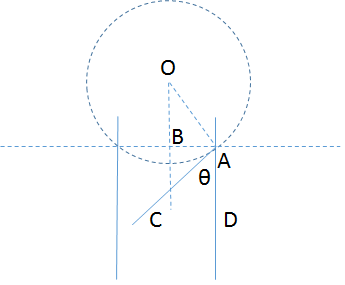
\includegraphics[scale=.5]{c1f1}}
\caption{Corresponding to figure 1.9.3 in the book}
\label{c1f1}
\end{figure}
We first observe that $\angle OAB = \theta$, therefore, $BA = OA\cos\theta$, or if $R$ is the radius of curvature then $a = R\cos\theta$. Therefore, the jump in pressure is
\[
\Delta p = \gamma\left(\frac{\cos\theta}{a} + \frac{\cos\theta}{a}\right) = \frac{2\gamma\cos\theta}{a}
\]
where $\Delta p = p_g - p_l$. Since $p_g$ is the atmospheric pressure, this indicates a pressure deficit in liquid. It is compensated by supporting a column of height $H$. Therefore,
\[
\Delta p = \rho g H
\]
so that
\[
\rho g H = \frac{2\gamma\cos\theta}{a}
\]
or
\[
H = 2\frac{\gamma}{\rho g}\frac{\cos\theta}{a}
\]
Using \eqref{c1s7e5},
\[
H = \frac{2d^2\cos\theta}{a}
\]

\item In the derivation of equation (1.9.7) in the book, consider a \enquote*{gaussian pillbox} of the kind used in electrodynamics.

\item In the analysis related to figure 1.9.4 the center of curvature is in the upper fluid. Therefore, the pressure rises while passing from the lower fluid to the upper. Or,
\begin{equation}\label{c1s7e7}
\sigma^\op_{ij}n_j - \sigma^\tp_{ij}n_j = \gamma\left(\frac{1}{R_1} + \frac{1}{R_2}\right)n_i
\end{equation}
\end{itemize}

\section{Exercises for the chapter}\label{c1s8}
\begin{enumerate}
\item We will first show that the excess pressure inside a bubble or radius $r$ is $4\gamma/r$, where $\gamma$ is the surface tension between liquid of which the bubble is formed. When a 
bubble of a liquid is created, its surface tension will try to minimize its surface area thereby compressing the gas inside. It will keep compressing the gas until a static equilibrium
between the pressure of the gas and surface tension is reached. Let us suppose that a bubble has reached this equilibrium stage. Imagine the bubble to be cut into two hemispheres. The 
upper hemisphere exerts a surface tension force of $2\times\gamma\times 2\pi r$, where $2\pi r$ is the perimeter of the hemisphere and we are multiplying by a factor of $2$ because there 
are two surfaces in a bubble, the outer and the inner. The upper hemisphere also exerts a pressure on the lower hemisphere. If $p$ is the excess pressure inside the bubble and $p_0$ is 
the ambient pressure, the force due to pressures is $(p-p_0)\times\pi r^2$. Under the condition of equilibrium, the pressure and the surface tension forces balance each other and we get 
an expression for the excess pressure $(p-p_0)$ inside a bubble as $4\gamma/r$.
\begin{rem}
If the bubble is replaced by a drop, the corresponding excess pressure will be half that of the bubble because a drop has only one surface unlike two in a bubble.
\end{rem}
First law of thermodynamics is $dU = \dbar{Q} + \dbar{W}$. In the process of coalescence of bubbles, there is no heat exchange, that is $\dbar{Q} = 0$. Further, $\dbar{W} = \dbar{pV} = 
Vdp + pdV$. Thus the energy change in coalescence of bubbles is $dU = Vdp + pdV$. If $p_0$ is the ambient pressure, the excess pressure inside a bubble of radius $a_1$ is 
\[
p = p_0 + \frac{4\gamma}{a_1}
\]
and that inside a bubble of radius $a_2$ is
\[
p = p_0 + \frac{4\gamma}{a_2}
\]
Thus, 
\[
Vdp = (4\gamma/a_1) \times (4\pi a_1^3/3)
\]
for a bubble of radius $a_1$. As the bubble grows from a volume $0$ to  $4\pi a_1^3/3$ under ambient pressure, the term $p\delta{V}$ for it is $p_0 4\pi a_1^3/3$. The energy needed to 
create the bubble of radius $a_1$ is
\begin{equation}\label{c1s8e1}
dU_1 = \frac{16\pi}{3}\gamma a_1^2 + \frac{4\pi}{3} a_1^3p_0
\end{equation}
Similarly, energy needed to create a bubble of radius $a_2$ is
\begin{equation}\label{c1s8e2}
dU_2 = \frac{16\pi}{3}\gamma a_2^2 + \frac{4\pi}{3} a_2^3p_0
\end{equation}
and the energy needed to create the coalesced bubble of radius $r$ is
\begin{equation}\label{c1s8e3}
dU = \frac{16\pi}{3}\gamma r^2 + \frac{4\pi}{3} r^3p_0
\end{equation}
Since at the end of the process of coalescence the temperature returns to that before, $dU = dU_1 + dU_2$. From \eqref{c1s8e1}, \eqref{c1s8e2} and \eqref{c1s8e3},
\[
p_0 r^3 + 4\gamma r^2=p_0(a_1^3 + a_2^3) + 4\gamma(a_1^2 + a_2^2)
\]

\item If there is no wetting, none of the liquid will stick to the sphere. The sticking happens because of a drop in pressure in the liquid. Since there is no more than a drop of liquid 
available, it forms a plano-concave lens with the plane along the rigid surface and concave portion along the spherical surface. The radius of curvature of the curved part of the plano-
concave lens is $a$. That of the plane part is infinity. Therefore, the interfacial pressure is
\[
p_l - p_g = \gamma\left(0 + \frac{1}{a}\right) = \frac{\gamma}{a},
\]
This excess pressure is distributed over the entire surface of the sphere, resulting in an adhesive force of
\[
4\pi a^2 \times \frac{\gamma}{a} = 4\pi\gamma a
\]

\item The problem asks us to explain apparent attraction and repulsion of floating bodies as a result of their wetting properties. Recent research shows that wetting properties 
\cite{vella2005cheerios} are not sufficient to explain the phenomenon.

An explanation that just takes into account the contact angle runs as follows. Imagine two floating bodies that have a wetting interface. Wetting causes the surface of water to rise
near the interface. Since the bodies prefer to float and are encouraged to do so by buoyancy, a neighboring body climbs up the rising interface giving an appearance of
attraction. Now let the two bodies have a non-wetting interface. The surface of water is now depressed and a neighboring floating body that also has a non-wetting interface, falls
along the depressed water surface once again giving appearance of attraction.

If one body, say $B1$, has a wetting interface and another, say $B2$ has a non-wetting interface, then the water surface is depressed around $B2$ and elevated around $B1$. If
$B1$ approaches $B2$, it prefers to slide up the interface due to its own buoyancy giving an appearance of repulsion.
\end{enumerate}

\section{Additional exercises}
\begin{enumerate}
\item \emph{Adhesive force between two plates wetted with a liquid}. Consider two plates with a small amount of liquid between them. If the liquid wets the plates, it will form a
convex meniscus of the type shown in figure \ref{c1f2}
\begin{figure}[!ht]
\centering
\centerline{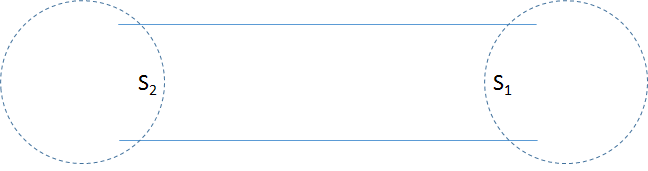
\includegraphics[scale=.5]{c1f2}}
\caption{Plates with a wetting liquid between them}
\label{c1f2}
\end{figure}
Since the center of curvature lies in the air, the excess pressure is in the air. Equivalently, there is a drop of pressure in the liquid. There is no more liquid available to rush
in the cavity to compensate the drop. Further, since the pressure is isotropic, there is a drop in pressure between the plates, resulting in a strong adhesion. At surface $S_1$, the
drop in pressure is
\[
\delta{p} = \gamma(R_1^{-1} + R_2^{-1}),
\]
where $R_1 = R_2 = a/\cos\theta$, $a$ being the separation between the plates. If $A$ is the area of the plate, then the force of adhesion is
\[
F = \frac{\gamma A \cos\theta}{a}
\]
Note that the same pressure drop is sufficient to sustain the surface $S_2$. We do not have to add it to the above expression.
\end{enumerate}